\section{Cognitive Impacts on the Ocular System} \label{sec:bt/cognitive_impacts}

As the reader might agree, vision may be the most vital sense of perception that humans enjoy. We can interpret vast amounts of information every second from the raw signals of millions of optic nerve fibers. This process is so complex that a significant fraction of the cortex is involved \cite{klatzky2012}. As such, it is natural to believe that our eyes are a good metric when studying the internal cognitive functions of our brain. In fact, the use of eye movements to learn from the inner workings of the mind has been exploited by cognitive psychologists for over two centuries \cite{wells1792}. 

This section will outline the most prominent impacts of cognition on the ocular system, where there are clear traces of correlation between the mind and the eyes. Some such correlations have clear causal links to neural circuitry and chemical release in the brainstem, while others can be determined by empirical evidence from clinical- and pharmacological studies.

% Some studies have even studied the possibility of inferring subject intention from their eye movements. \cite{ballard1992}, for instance, wanted to investigate whether gaze patterns were an indicator that preceded actions. To do this, he conducted an experiment where subjects were to move a set of colored blocks to match the pattern of a given model, while a mobile eye tracker was set up to record their eye movements. He found that there was indeed a strong link between a subject's eye movements and their actions. Gaze followed a clear pattern of checking out a block before picking it up and the model before placing it down. Similarly, \cite{land1999} measured a subject's eye movements as they performed daily tasks, such as brewing tea or making a sandwich, again finding that the subject's eyes always revealed their intentions before acting.

\subsection{Pupillometry} \label{sec:bt/cognitive_impacts/pupillometry}

Voluntary effort drives visual perception. Except for reflexive responses, eye movements require conscious activation of the extraocular muscles surrounding the eyes. These are necessary movements for placing visual information on the retina and are well-understood. Even after attention is directed at an object, other eye movements constantly operate to provide our brain with an optimal image of reality. One such operation includes lens stretching to provide focused light from near and far objects. Another is responsible for light admission to the retina by constricting and dilating the pupil. From a neurological examinator's standpoint, the latter is of particular interest. Pupillometry is the study of pupil size and reactivity and will be further elaborated on in the current subsection.

% shifts in attention between objects must be done by consciously activating the extraocular muscles surrounding the eye.

Our brain regulates pupil diameter as a response to three distinct types of stimuli. Brightness and near fixations constrict its size, and cognitive activity dilates it. These types of stimuli will be referred to as the \acrfull{plr}, \acrfull{pnr} and \acrfull{ppr}, respectively. Although not particularly interesting in the larger context of this thesis, the effects of \acrshort{plr} and \acrshort{pnr} must still be understood when assessing the cause of a given pupillary response. 

\subsubsection{\acrfull{plr} and \acrfull{pnr}} \label{sec:bt/cognitive_impacts/plr_pnr}

Average pupil size ranges from 1.5mm in bright lighting to 9mm in total darkness \cite{eckstein2017}. The physiological explanation for this effect is clear: A large pupil allows for more light to fall on the retina, thus increasing the amount of information sent to the brain at any time. Photoreceptors on the retina quickly become saturated upon bright light exposure, rendering them less sensitive. Subsequent exposure to faint objects in dim light requires dark adaptation, taking tens of minutes. During this time, vision is substantially impaired. To avoid this issue, the pupil may rapidly dilate upon changing environments from bright to dim, effectively acting as a buffer for light admittance. This behavior is subconsciously controlled by the \acrshort{plr}.

Diverting gaze between near and far objects causes an additional few millimeters of changes in pupil size. This response is explained by optical distortion of light passing through the lens, caused by \textit{spherical aberration}. This distortion occurs because the light entering an aperture is increasingly refracted toward the edges of a convex lens, causing rays not to converge on the same focal point. The effect is illustrated in figure \ref{fig:bt/spherical_aberration}. Like with a conventional camera, less spherical aberration means that deeper planes of the visual field may be in focus simultaneously. Reducing the amount of light that has to enter through the lens edges by reducing the aperture size, therefore, deepens the field of focus.

Furthermore, since focusing on closer objects require a rounder lens causing even more distortion, optimal vision at close range benefits from a constricted pupil. As with the \acrshort{plr}, this behavior is subconsciously controlled by the \acrshort{pnr}.

\begin{figure}[h]
    \centering
    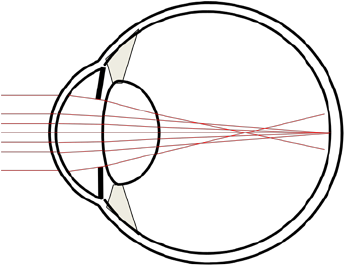
\includegraphics[width=0.6\textwidth]{figures/bt_spherical_aberration.png}
    \caption{Simplified illustration of spherical aberration in the eye. Light passing through the outer edges of the lens are refracted to a larger degree than those passing through the center, causing image distortion. }
    \source{\cite{huang2011}}
    \label{fig:bt/spherical_aberration}
\end{figure}

Whereas both the \acrshort{plr} and the \acrshort{pnr} can cause pupil size to vary by half or double its original size, \acrshort{ppr} only accounts for changes of less than 0.5mm \cite{beatty1982}. Naturally, this leads to significant sources of bias if the cognitively evoked responses are what we are interested in measuring. Researchers may mitigate the effects of \acrshort{pnr} by keeping the stimulus at a constant distance from the subject, which is usually the case for most studies that present stimuli on a computer monitor. To account for the \acrshort{plr}, studies suggest moderately and constantly lit environments \cite{steinauer2004}. By closely controlling these two factors and recording a baseline pupil diameter for each subject, researchers may observe the \acrshort{ppr} by measuring deviations from this baseline. 
% Experiments conducted in this thesis will therefore present stimuli on a monitor with the subject at a fixed distance from the screen, in a room with moderate lighting.

% In the right conditions, however, the effects of both \acrshort{plr} and \acrshort{pnr} may be largely mitigated. 




% Although the \acrshort{plr} is mostly reflexive in nature, it has been shown to be modestly affected by cognitive influences as well. For instance, some studies show that even covert attention to bright objects cause pupil contraction even before bright light hits the retina.

\subsubsection{\acrfull{ppr}}

While the \acrshort{plr} and the \acrshort{pnr} offer rather clear-cut causes for their effect (e.g. light intensity or distance to fixation), the \acrshort{ppr} is not that simple. One cannot link pupil size to just one cognitive process. A multitude of mental mechanisms, such as alertness, arousal, mental effort, and cognitive capacity, have all been linked to pupil dilation in some way \cite{beatty1982, just2003, andreassi2000}. \textcite{eckstein2017} states that "pupil dilation reflects a specific, intensity- and attention-related aspect of cognitive processing."
% What can be clearly stated, however, is that. "pupil dilation reflects a specific, intensity- and attention-related aspect of cognitive processing." \cite{eckstein2017}. 
In other words, any cognitive process that requires heightened attention or deliberate effort will affect pupil size.

Two distinct central- and autonomous nervous system pathways govern pupil dilation and constriction. One is responsible for the fight-or-flight response and is referred to as the \acrfull{sns}. The other is called the \acrfull{pns} and controls what is known as the rest-and-digest response \cite{blessing2008}. As their responses might suggest, they operate under entirely different circumstances. When chemicals in the brainstem stimulate the \acrshort{sns}, heart rate, sweat- and glucose production is accelerated, and pupils dilate. Conversely, stimulation of the \acrshort{pns} will constrict the pupil, slow the heartbeat, and trigger digestion, secretion, and voiding. This connection hints at why pupils are small at rest and larger when aroused or agitated.

Furthermore, there is a cluster of neurons in our brain called the \acrfull{lc}. These neurons have shown direct inhibitory projections with the \acrshort{pns} and excitatory projections with the \acrshort{sns} \cite{eckstein2017}. In other words, increased activity in the \acrshort{lc} triggers bodily functions associated with fight-or-flight while halting those associated with rest-and-digest. These responses further lead to reduced activation of the pupil's constricting fibers and increased activation of its dilating fibers, thus increasing its size. A study by \textcite{rajkowski1993} demonstrated this effect, where they recorded neuronal \acrshort{lc} activity in monkeys during a target detection task. During this task, monkeys were made to exert different levels of effort over time. As is evident from figure \ref{fig:bt/lc_corr}, a striking temporal coupling between \acrshort{lc} activity and pupil size was shown. 

\begin{figure}[h]
    \centering
    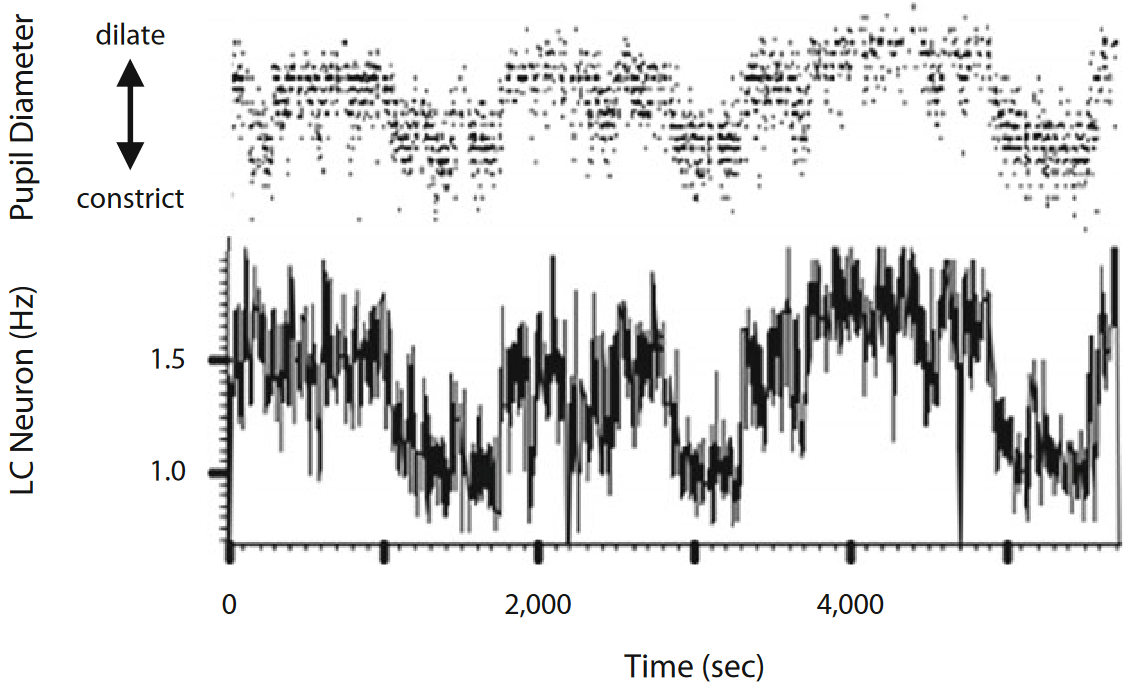
\includegraphics[width=0.8\textwidth]{figures/bt_LC_correlation.png}
    \caption{\acrlong{lc} firing rate (bottom) and pupil diameter in monkeys (top). Demonstrates clear connection between \acrshort{lc} and \acrshort{pns} inhibition, which we know regulates pupil diameter.}
    \source{\cite{rajkowski1993}}
    \label{fig:bt/lc_corr}
\end{figure}

To explain why the \acrshort{ppr} has any coupling with cognition, besides being associated with the fight-or-flight response, we need to understand the \acrlong{lc}. Studies show that the \acrshort{lc} plays a critical role in physiological arousal and cognitive functioning. In fact, the \acrshort{lc} is the only source of \acrfull{ne} in the cerebral cortex \cite{sara2009}. \acrshort{ne}, synthesized from \acrfull{da}, is an essential neuromodulator of brain activity \cite{aminoff2014}. Although it produces many effects in the body, the most notable is boosting the signal-to-noise ratio of incoming sensory information. 

This effect has been demonstrated in spatial working memory tasks in monkeys, where chemicals that inhibited \acrshort{ne} release was administered to observe their effect on task performance. The task given was to search through a number of boxes and find target objects. In subsequent trials, the monkeys were rewarded for remembering previous targets. The neural circuitry of working memory associated with the target responses had increased activation with higher levels of \acrshort{ne}. Conversely, activation of the neural circuitry surrounding this particular response was reduced \cite{ramos2007}. In other words, the monkey was more likely to select a response corresponding to the target when \acrshort{ne} release was higher. Higher firing rates of the \acrshort{lc} therefore made "signals" from the neural circuitry corresponding to the target response strengthened compared to the "noise" from incorrect responses.

In summary, research shows that we can use \acrshort{ne} quantities in the brainstem as a measure of how narrow or broad the attentional focus is. Attentional focus may encapsulate a variety of complex cognitive functions, such as mental workload, working memory capacity, decision making, and much more \cite{sara2009}. Since \acrshort{ne} is directly mediated by the \acrfull{lc}, which has neural links with segments of the central nervous system governing pupil size, \acrshort{ppr} may be used as a proxy for such cognitive functions.

% Neural circuitry in the pre-frontal cortex has the ability to represent visual information even after it has been represented. It is therefore thought to be represent the physiological basis for working memory.

\subsubsection{Experiments}

A famous experiment by \textcite{kahneman1966} was one of the first which demonstrated pupillometry as a measure of cognition. In this study, pupil diameter was shown to reflect the amount of material that was under active processing at any time. They employed several short-term memory tasks, one of which is reproduced in figure \ref{fig:bt/pupillary_expA}. For this particular task, strings of varying lengths of digits were presented to the subject. After a two-second pause, they were instructed to repeat them from memory. Naturally, longer strings imposed a higher load on working memory than shorter ones. This relation shows a significant correlation with average pupil diameter. Interestingly, the pupil seems to dilate for every new digit presented, peaking just before recall begins. The pupil then constricts for every digit recalled, returning to baseline after the task is completed. 
% This study demonstrate characteristics of the task-evoked pupillary response, 

In addition to this task-evoked response, another experiment by \textcite{hopstaken2015} also demonstrate that cognitive load markedly affects the pupil diameter baseline. This study employed the N-back task, a task which will be explained in much more detail in section \ref{sec:impl/tasks}. In short, it is designed to be simple in principle and very cognitively demanding in practice. It requires the sustained engagement of working memory and attention at varying difficulty levels from simple (0-back) to very hard (3-back). As is apparent from figure \ref{fig:bt/pupillary_expB}, baseline pupil diameter was consistently larger with increased task difficulty. This experiment also demonstrates how fatigue from continued task exposure affects task engagement. Each time-on-task block on the x-axis represents 18 minutes of task exposure. As is evident from the decrease in baseline pupil diameter for each block, task exposure also has a noticeable effect on pupil size. This relation could, in theory, be leveraged as an indicator of task engagement or mental fatigue.

\begin{figure}[h]
    \begin{subfigure}[b]{0.5\textwidth}
        \centering
        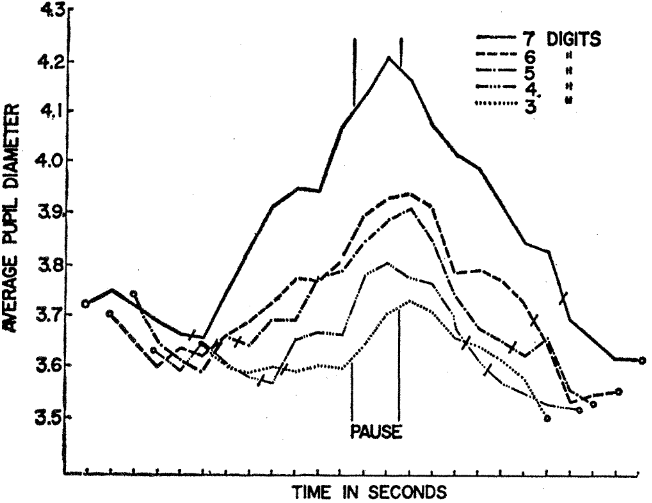
\includegraphics[width=\textwidth]{figures/bt_kahneman1966.png}
        \vspace{0.5mm}
        \caption{}
        \label{fig:bt/pupillary_expA}
    \end{subfigure}
    \begin{subfigure}[b]{0.5\textwidth}
        \centering
        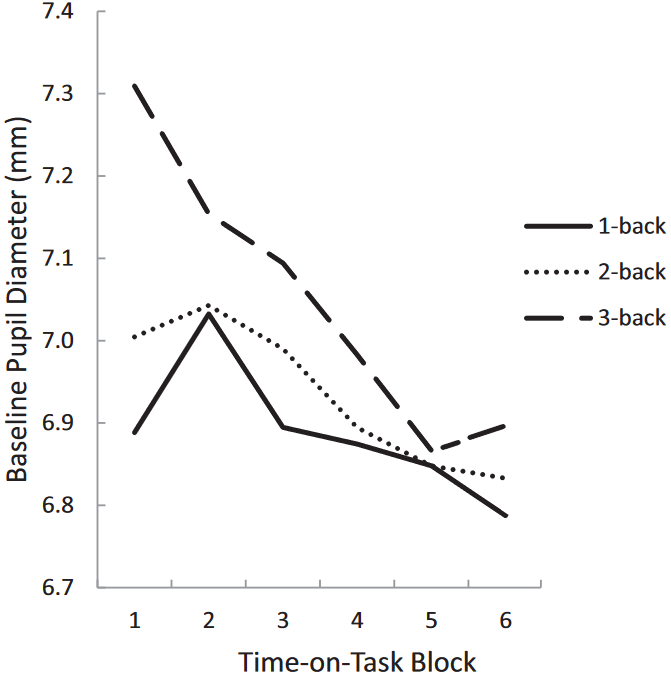
\includegraphics[width=\textwidth]{figures/bt_hopstaken2015.png}
        \caption{}
        \label{fig:bt/pupillary_expB}
    \end{subfigure}
    \caption{\textbf{a)} Average pupil diameter during a short-term memory task. Each line represent one length of string for recall. Tick marks before and after the pause indicate the beginning of string presentation and end of recall, respectively. Points are calculated from an average over all subjects at one time instance. \textbf{b)} Average baseline pupil diameter during three difficulty levels of the n-back task. Each graph represent one value of N (i.e., task difficulty level). Points are calculated from an average of all subjects and all time instances during 6 minutes of task exposure for each difficulty level.}
    \source{\cite{kahneman1966, hopstaken2015}}
\end{figure}

% Pupil dilation in response to arousal. Dilated pupils are subconciously perceived as more attractive.

\newpage
\subsection{\acrfull{ebr}} \label{sec:bt/cognitive_impacts/ebr}

Another well-understood ocular event is blinking. It serves eye health by distributing an even layer of moisture across the eyeball and protects against foreign objects by reflexive closure. Contrary to the pupillary response, blinking can be controlled by conscious effort. Therefore, when considering the cognitive implications of blink rate, we need to define \textit{spontaneous eyeblinks}. What characterizes these eyeblinks is that cognitive functions subconsciously induce them without interference from volition. They differ from reflexive eyeblinks because they occur at predictable rates and without the triggers of foreign objects.

% Both such events are of little interest, however, as they have little correlation with cognition. A third form of eyeblinks are classified as \textit{spontaneous eyeblinks}, and will be the focus of this subsection. Like reflexive eyeblinks, spontaneous eyeblinks occur without volition. What characterizes them, however, is that they arise without the triggers of foreign objects and at a somewhat constant rate during all activities.

\acrfull{ebr}, the rate at which spontaneous eyeblinks occur, is a reliable measure of \acrfull{da} activity in the central nervous system. Although the precise neural circuitry that controls blink rate is primarily unknown \cite{eckstein2017}, empirical studies have repeatedly demonstrated this relationship.


\acrshort{da} activity in both human and non-human primates can reliably be observed by either pharmacological manipulations or from clinical studies. For instance, administration of the well-known \acrshort{da} agonists \textit{apomorphine} and \textit{amphetamine} have shown statistically significant increases in \acrshort{ebr} in both humans \cite{blin1990, strakowski1998, strakowski1996}, and monkeys \cite{redmond2011, kotani2016}. Apomorphine effect on \acrshort{ebr} is shown in figure \ref{fig:bt/da_corr}. Similarly, many conditions are known to affect the dopaminergic system. One such condition is Parkinson's disease, a disorder caused by a loss of dopaminergic cells in some parts of the brain. Patients suffering from Parkinson's show a significantly reduced \acrshort{ebr} compared to healthy individuals \cite{bologna2012}. Other conditions, such as schizophrenia and Tourette's syndrome, are linked with elevated \acrshort{da} activity and show increased \acrshort{ebr}. 

\begin{figure}[h]
    \centering
    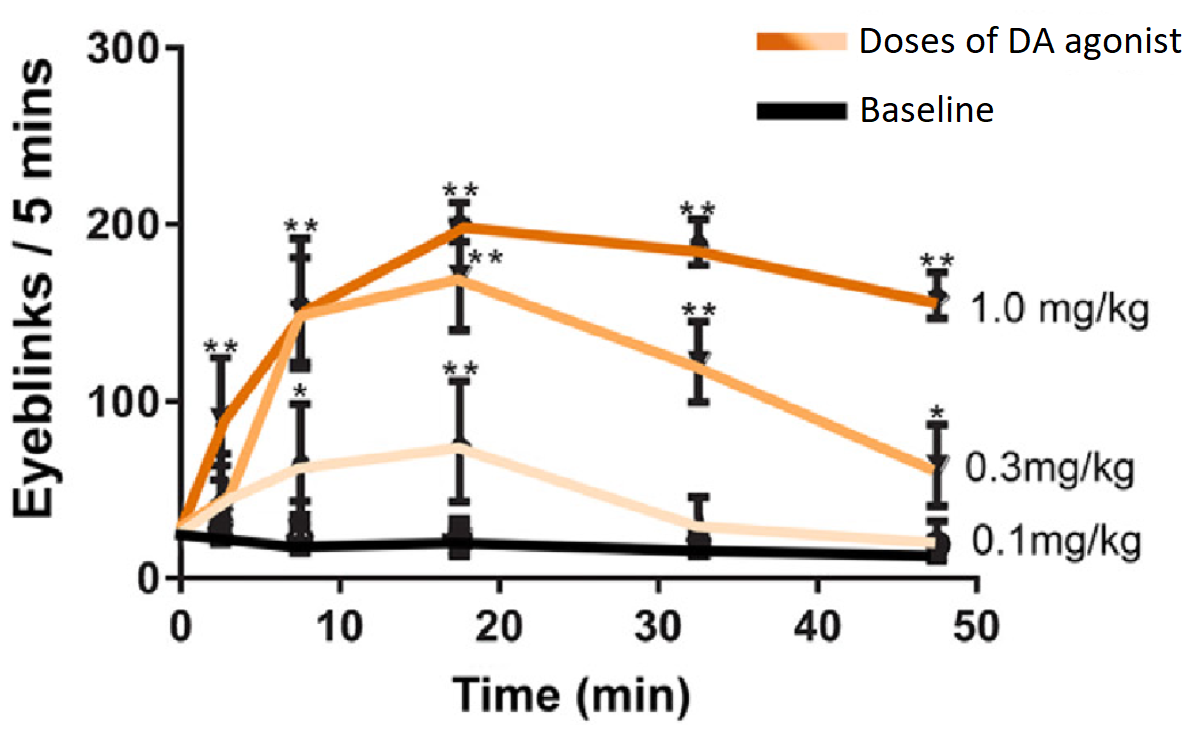
\includegraphics[width=0.8\textwidth]{figures/bt_DA_correlation.png}
    \caption{\acrlong{ebr} for three dosages of DA agonist apomorphine against baseline (no pharmacological manipulation). Note that \acrshort{ebr} values on y-axis show deviations from baseline, hence why baseline graph is constantly at 0.}
    \source{\cite{kotani2016}}
    \label{fig:bt/da_corr}
\end{figure}

Just like \acrshort{ne}, \acrshort{da} is an important neuromodulator for brain activity. Especially for learning and \textit{cognitive control}, \acrshort{da} activity has shown to be an important aggregator. Cognitive control is a term that broadly describes our ability to control impulses, maintain goals and focus on specific tasks without diverting attention. Research in this area has shown a near positive-linear relationship between baseline \acrshort{da} levels in the brainstem and cognitive control in goal-oriented tasks \cite{puig2014, westbrook2016}. In addition to baseline levels, phasic \acrshort{da} activity has shown positive correlations with changing task environments. \textcite{bochove2012}, for instance, showed that an increased \acrshort{ebr} in one task trial could reliably predict the level of cognitive control and performance in the subsequent trial.

% Empirical studies with clinical samples

\subsubsection{Experiments}

A classic experiment to ascertain cognitive control is called the Stroop test. It is set up such that the subject is presented with a series of words representing colors (e.g., red, green, blue). Each word stimulus is said to be \textit{congruent} if the font color matches the word. If colors do not match, the stimulus is \textit{incongruent}. Incongruent stimuli are notably challenging since the subject is presented with two conflicting visual inputs, and an intuitive answer does not come to mind without some thought. Numerous studies, including the original by \textcite{stroop1935}, show that the incongruent condition causes an increased response time of about 75\% compared to the congruent condition. More recent studies suggest that conflicts in the word read and the color seen requires higher levels of cognitive control to respond correctly \cite{egner2005, bugg2012}. 

An experiment by \textcite{oh2012} employed the Stroop test to examine task-evoked \acrshort{ebr}, similar to \textcite{bochove2012}. In this study, subjects were presented with 60 randomly distributed congruent and incongruent stimuli. Each stimulus stayed on-screen for two seconds or until the subject responded with a color. They found that, of the 27 subjects in the experiment, each subject could be divided into distinct subgroups based on their eyeblink behavior when responding. Seventeen showed a consistent tendency to blink directly before responding (subgroup I), and seven directly after (subgroup II). Four subjects showed both behaviors (subgroup III). As can be seen from figure \ref{fig:bt/oh2012A}, eyeblinks were much more likely to occur in the $\pm$500ms surrounding the subject response. 
% The effect was even more pronounced subgroups I and II
Subgroups I and II demonstrated this effect even more clearly, and together, they represent an 88\% majority. For all three subgroups, this suggests that spontaneous eyeblinks are closely associated with the exertion of cognitive control and may signal a shift in the subjects' internal cognitive or attentional state.

\begin{figure}[h!]
    \centering
    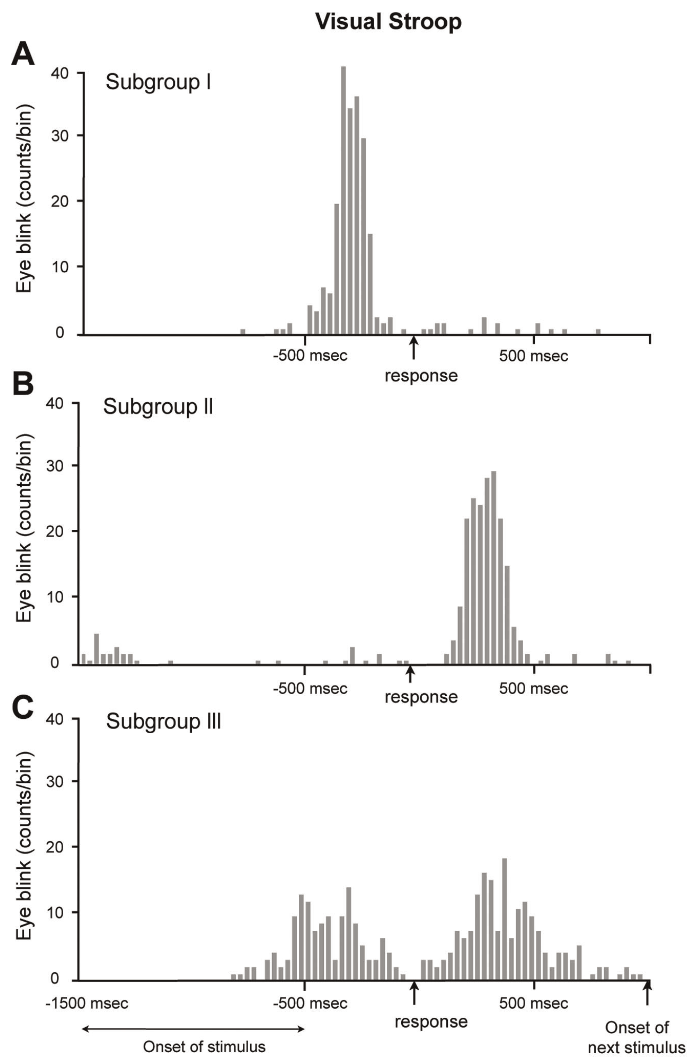
\includegraphics[width=0.8\textwidth]{figures/bt_oh2012A.png}
    \caption{Histogram showing spontaneous eyeblink count as a response to the Stroop test. Each bin (point on the x-axis) represents 30-millisecond intervals. An arrow indicates the time of response. Due to randomness, stimulus onset is between -1500ms and -500ms from the response. Onset of the next stimulus occurs after a one seconds waiting period.}
    \source{\cite{oh2012}}
    \label{fig:bt/oh2012A}
\end{figure}

During the same study by \textcite{oh2012}, baseline \acrshort{ebr} levels were measured during a two-minute resting period both between trials and on-task. As can be seen from figure \ref{fig:bt/oh2012B}, the color-naming task produced a slightly higher \acrshort{ebr} than the word-reading task. Furthermore, the average on-task \acrshort{ebr} turned out to be almost 50\% elevated from the resting baseline. These results suggest that \acrshort{ebr} may not only indicate shifts in cognitive control but also sustained attention.

\begin{figure}[h!]
    \centering
    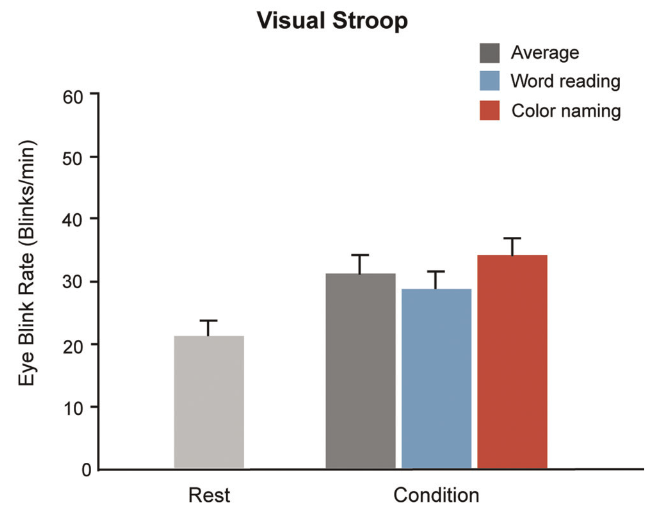
\includegraphics[width=\textwidth]{figures/bt_oh2012B.png}
    \caption{\acrfull{ebr} during the Stroop test. The resting eyeblink rate in light grey was recorded during a 2 minute long idle period between trials. Word reading and word naming conditions represent trials where the target response was the word of the stimulus and the color of the stimulus, respectively.}
    \source{\cite{oh2012}}
    \label{fig:bt/oh2012B}
\end{figure}

\subsection{Eye Gaze} \label{sec:bt/cognitive_impacts/gaze}

Eye gaze comprises all voluntary and involuntary eye movements besides those mentioned above. Fixations, saccades, and microsaccades are examples, but so are all features that they induce: Saccadic frequency, fixation duration, field-of-view, and so on. Although voluntary in nature, many of these elements are in reality governed by subconscious cognitive aspects. It is these correlations we will attempt to uncover in this subsection. As for the spontaneous eyeblink rate, the neural circuitry underlying these events is difficult to pinpoint. There are, however, empirical studies that show promising correlations.

\newpage
\subsubsection{Experiments}

A series of interesting studies by \textcite{williams1982, williams1985, williams1988} suggest that task-induced cognitive load may adversely affect the subject's field of view, as measured by information perceived in the visual periphery. Such results are hard to measure accurately, as gaze patterns are immensely complex and may introduce significant confounding variables. He employed a task where subjects were required to report the orientation of lines presented at varying distances from a fixation point. At central vision, they were required to perform a short-term memory task with varying levels of induced cognitive load. \textcite{williams1985} found that the accuracy of determining line orientation deteriorated rapidly with increasing cognitive load in the primary task. He argues that this suggests a human tendency to subdue our field of view when highly concentrated or under a heavy mental workload.

Another study by \textcite{underwood1997} demonstrated that varying levels of cognitive demand during a driving task affected the individual's search patterns. They managed this by instructing a group of subjects to drive a car through a set route, during which their eye movements would be recorded for three separate one-minute intervals. The intervals were designed to represent three levels of demand based on the type of road they were on. One was a one-lane rural road with good visibility. Another was a busy suburban road with much traffic and pedestrians. The third was a high-speed dual-carriageway joined by two slip roads from the left and right. 

As can be seen from the results presented in figure \ref{fig:bt/underwood1997}, the types of roads significantly affect fixation durations and both vertical and horizontal search patterns. It seems that fixation durations decrease on the more demanding roads while the search strategy widens, indicating a cognitive effect on gaze. These results are reasonable, as shorter duration and more frequent fixations are naturally associated with heightened awareness. The wider search patterns are also natural since demanding roads require attention to the information in a larger field of view.

The same study by \textcite{underwood1997} also researches the effect of experience on search patterns. 
% That discussion is beyond the scope of this section. However, i
It is interesting to note that while experienced drivers expand their field of view when encountering the more demanding roads, novice drivers tend to maintain one level of scanning throughout. 
This result relates to the theory derived in section \ref{sec:bt/CLT/domains}, which connects experience with the construction of mental schemas. Such schemas allow for fewer demands on working memory, which is subsequently apparent in gaze patterns.
% By additionally controlling for differences between experienced and inexperienced drivers, they were able to show that schema construction have real implications on the cognitive load induced by a task.

\begin{figure}[h]
    \centering
    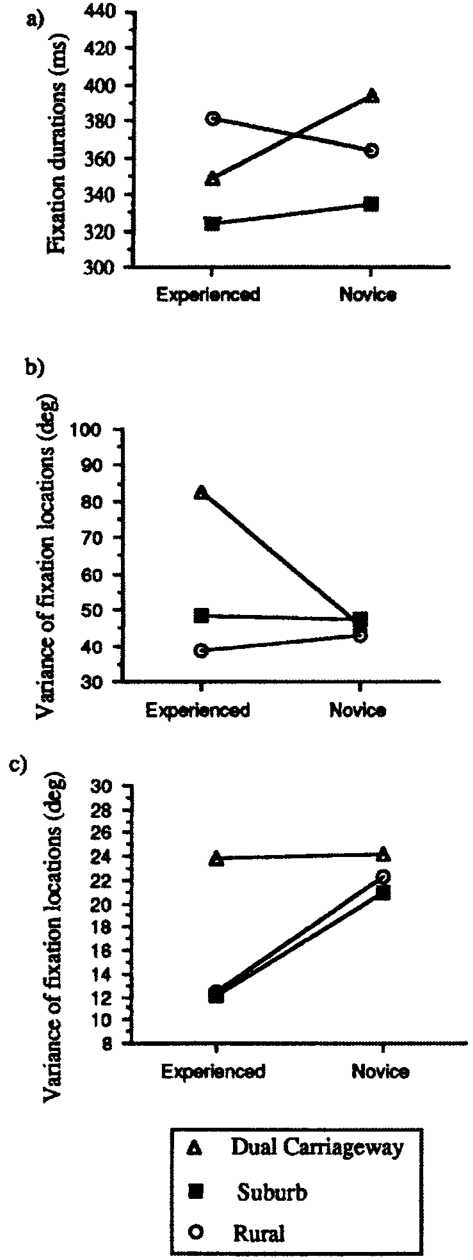
\includegraphics[width=0.6\textwidth]{figures/bt_underwood1997.png}
    \caption{Gaze patterns observed on subjects in a driving task. Each plot is labeled by the type of road driven on. Each road type infers differing levels of demand from the driver. \textbf{a)} Mean fixation durations. \textbf{b)} Horizontal variance in fixation locations \textbf{c)} Vertical variance in fixation locations.}
    \source{\cite{underwood1997}}
    \label{fig:bt/underwood1997}
\end{figure}

\FloatBarrier